\documentclass[11pt,a4paper]{article}

\usepackage[utf8]{inputenc}
\usepackage[T1]{fontenc}
\usepackage{lmodern}
\usepackage[margin=0.82in]{geometry}
\usepackage[table]{xcolor}
\usepackage{array}
\usepackage{tabularx}
\usepackage{booktabs}
\usepackage{enumitem}
\usepackage{titlesec}
\usepackage{fancyhdr}
\usepackage{lastpage}
\usepackage{hyperref}
\usepackage{tikz}

\definecolor{TextInk}{HTML}{233142}
\definecolor{HeadingBlue}{HTML}{1D3557}
\definecolor{AccentTeal}{HTML}{2A7F92}
\definecolor{AccentGold}{HTML}{C58B4E}
\definecolor{RuleGray}{HTML}{D6E0E5}
\definecolor{TableStripe}{HTML}{F3F8FA}
\definecolor{SoftTint}{HTML}{F7F4EE}
\definecolor{SoftBlue}{HTML}{EEF6F8}
\definecolor{SoftGreen}{HTML}{EEF7F0}
\definecolor{SoftRed}{HTML}{FBF0EF}

\hypersetup{
  colorlinks=true,
  linkcolor=HeadingBlue,
  urlcolor=AccentTeal,
  pdftitle={IB Geography SL Study Pack - 2026-04-25},
  pdfauthor={IB Geography SL Preparation}
}

\color{TextInk}
\setlength{\parskip}{0.52em}
\setlength{\parindent}{0pt}
\setlength{\tabcolsep}{6pt}
\renewcommand{\arraystretch}{1.22}
\setlist[itemize]{leftmargin=1.35em,itemsep=3pt,topsep=4pt}
\setlist[enumerate]{leftmargin=1.5em,itemsep=3pt,topsep=4pt}

\newcolumntype{Y}{>{\raggedright\arraybackslash}X}
\newcolumntype{L}[1]{>{\raggedright\arraybackslash}p{#1}}

\titleformat{\section}
  {\normalfont\huge\sffamily\bfseries\color{HeadingBlue}}
  {}{0pt}{}
  [\vspace{0.15em}{\color{AccentGold}\titlerule[1pt]}]

\titleformat{\subsection}
  {\normalfont\Large\sffamily\bfseries\color{AccentTeal}}
  {}{0pt}{}

\titleformat{\subsubsection}
  {\normalfont\large\sffamily\bfseries\color{HeadingBlue}}
  {}{0pt}{}

\titlespacing*{\section}{0pt}{1.4em}{0.65em}
\titlespacing*{\subsection}{0pt}{1.0em}{0.35em}
\titlespacing*{\subsubsection}{0pt}{0.8em}{0.25em}

\pagestyle{fancy}
\setlength{\headheight}{14pt}
\fancyhf{}
\fancyhead[L]{\sffamily\color{AccentTeal}Sat 2026-04-25}
\fancyhead[R]{\sffamily\color{HeadingBlue}IB Geography SL}
\fancyfoot[C]{\sffamily\color{HeadingBlue}\thepage\ of \pageref{LastPage}}
\renewcommand{\headrulewidth}{0.4pt}
\renewcommand{\footrulewidth}{0pt}

\newcommand{\term}[1]{\textcolor{HeadingBlue}{\textbf{#1}}}
\newcommand{\exam}[1]{\textcolor{AccentTeal}{\textbf{#1}}}
\newcommand{\boxnote}[3]{%
\noindent\colorbox{#1}{%
  \begin{minipage}{0.965\textwidth}
  \sffamily
  \textbf{\textcolor{HeadingBlue}{#2}} #3
  \end{minipage}
}}

\begin{document}

\begin{center}
  {\sffamily\bfseries\color{HeadingBlue}\LARGE IB Geography SL Study Pack}\\[0.25em]
  {\sffamily\bfseries\color{AccentTeal}\Large Saturday 2026-04-25}\\[0.35em]
  {\sffamily\color{TextInk}Urban Environments Depth: Recall, Timed Practice, Marking, And Precision Drill}
\end{center}

\vspace{0.5em}

\boxnote{SoftBlue}{How this pack follows the plan.}{The April 25 schedule is a
weekend \term{90 minute} session: \term{30 minutes} closed-book recall of Urban
environments, land-use patterns, urbanization, migration, and named examples;
\term{30 minutes} of Paper 1 structured-question style practice;
\term{20 minutes} to mark and log errors; and \term{10 minutes} to drill
numbers, place names, and definitions. This pack is designed for direct PDF
conversion with a textbook-style color scheme and printable tables.}

\section{Today's Target}

By the end of this session, you should be able to:

\begin{itemize}
  \item recall the four main Urban environments subtopic clusters without notes
  \item describe common urban land-use patterns and explain why they form
  \item connect \term{urbanization} and \term{migration} to housing, service,
  employment, and environmental pressures
  \item use two or three named examples with enough precision for a timed answer
  \item answer one structured Paper 1 style practice set under time
  \item mark your own answer by command term, evidence, explanation, and
  evaluation
\end{itemize}

\subsection{90-Minute Session Map}

\rowcolors{2}{TableStripe}{white}
\begin{tabularx}{\textwidth}{L{0.16\textwidth}Y L{0.24\textwidth}}
\toprule
\textbf{Time} & \textbf{Task} & \textbf{Output} \\
\midrule
0--30 min & Closed-book recall of Urban environments, land-use patterns,
urbanization, migration, and examples & One completed recall map \\
30--60 min & Timed structured-question practice & One full practice response \\
60--80 min & Self-mark, compare with the marking guide, and write an error log
& Three fixes to carry forward \\
80--90 min & Drill numbers, place names, and definitions & At least ten precise
facts or terms checked \\
\bottomrule
\end{tabularx}
\rowcolors{2}{}{}

\section{30-Minute Recall Block}

\subsection{The Four-Cluster Map}

Before reading further, shut the pack and write the four clusters from memory.
Then reopen and check against this list:

\begin{enumerate}
  \item \term{Variety of urban environments and urban spatial patterns}
  \item \term{Changing urban systems}
  \item \term{Urban environmental and social stresses}
  \item \term{Building sustainable urban systems for the future}
\end{enumerate}

These four clusters stop Urban environments from becoming a loose list of city
facts. Use them as the first sorting system in every answer. If a question asks
about land value, housing zones, central business districts, or informal
settlement location, it belongs mainly in \term{spatial patterns}. If it asks
about urbanization, migration, suburbanization, counter-urbanization,
reurbanization, megacity growth, gentrification, or deindustrialization, it
belongs mainly in \term{changing urban systems}. If it asks about air pollution,
congestion, waste, inequality, housing shortage, or segregation, it belongs in
\term{urban stress}. If it asks about transport planning, green space,
affordable housing, waste management, or future cities, it belongs in
\term{sustainable management}.

\subsection{Urban Land-Use Patterns}

Urban land use means how different functions are arranged across a city. The
most important exam habit is to move from \term{pattern} to \term{process}.
Do not only say where things are. Say why they are there.

\rowcolors{2}{TableStripe}{white}
\begin{tabularx}{\textwidth}{L{0.23\textwidth}Y Y}
\toprule
\textbf{Land-use feature} & \textbf{Typical pattern} & \textbf{Process that can explain it} \\
\midrule
Central business district & Highly accessible central zone with offices,
retail, high land values, and strong transport links & Competition for the most
accessible land raises rent and encourages high-density commercial use \\
Inner city & Older housing, former industry, transport nodes, and possible
reinvestment or decline & Industrial history, deindustrialization,
reurbanization, and gentrification reshape the area over time \\
Suburbs & Lower-density residential areas, often with more private space and
car-dependent travel & Suburbanization, road building, household income, and
preference for larger homes can push growth outward \\
Rural-urban fringe & Mixed land use at the city edge: housing estates,
warehouses, roads, retail parks, and remaining farmland & Urban expansion and
cheaper peripheral land create pressure on agricultural and greenfield sites \\
Informal settlement & High-density housing on marginal or insecure land, often
with weak service access & Rapid urbanization, poverty, housing shortage, and
limited formal planning can force self-built settlement \\
Edge city or secondary center & Retail, offices, and services away from the
traditional city center & Decentralization, car access, land availability, and
business demand create new nodes \\
\bottomrule
\end{tabularx}
\rowcolors{2}{}{}

\subsection{How To Use Land-Use Models}

Classic land-use models are useful, but they are not answers by themselves.
Use them as \term{thinking tools}, then evaluate their limits.

\begin{itemize}
  \item \term{Burgess concentric model}: land uses form rings around a central
  business district. It helps explain distance decay from the center, but it can
  oversimplify modern cities with multiple centers and uneven transport routes.
  \item \term{Hoyt sector model}: land uses grow outward in sectors along
  transport routes. It helps explain industrial corridors or high-income
  residential wedges, but it may not fit cities shaped by informal growth or
  strong planning controls.
  \item \term{Multiple nuclei model}: cities have several centers of activity.
  It is useful for large, decentralized, car-based, or polycentric urban
  regions, but it still needs local evidence.
\end{itemize}

\subsubsection{Quick Model Sketches}

\begin{center}
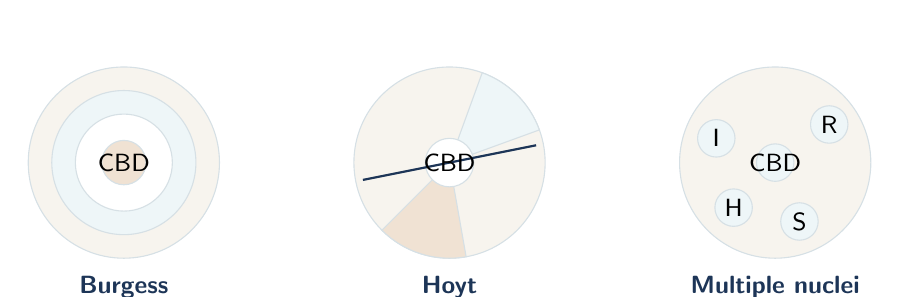
\begin{tikzpicture}[scale=0.88, every node/.style={font=\sffamily\small}]
  \begin{scope}
    \draw[fill=SoftTint, draw=RuleGray] (0,0) circle (1.38);
    \draw[fill=SoftBlue, draw=RuleGray] (0,0) circle (1.04);
    \draw[fill=white, draw=RuleGray] (0,0) circle (0.70);
    \draw[fill=AccentGold!25, draw=RuleGray] (0,0) circle (0.32);
    \node[font=\sffamily\bfseries\small, color=HeadingBlue] at (0,-1.8) {Burgess};
    \node at (0,0) {CBD};
  \end{scope}
  \begin{scope}[xshift=4.7cm]
    \draw[fill=SoftTint, draw=RuleGray] (0,0) circle (1.38);
    \draw[fill=SoftBlue, draw=RuleGray] (0,0) -- (20:1.38) arc (20:70:1.38) -- cycle;
    \draw[fill=AccentGold!25, draw=RuleGray] (0,0) -- (225:1.38) arc (225:280:1.38) -- cycle;
    \draw[fill=white, draw=RuleGray] (0,0) circle (0.35);
    \draw[HeadingBlue, thick] (-1.25,-0.25) -- (1.25,0.25);
    \node[font=\sffamily\bfseries\small, color=HeadingBlue] at (0,-1.8) {Hoyt};
    \node at (0,0) {CBD};
  \end{scope}
  \begin{scope}[xshift=9.4cm]
    \draw[fill=SoftTint, draw=RuleGray] (0,0) circle (1.38);
    \foreach \x/\y/\name in {0/0/CBD,0.78/0.55/R,-0.85/0.35/I,0.35/-0.85/S,-0.6/-0.65/H}
      \draw[fill=SoftBlue, draw=RuleGray] (\x,\y) circle (0.27) node {\name};
    \node[font=\sffamily\bfseries\small, color=HeadingBlue] at (0,-1.8) {Multiple nuclei};
  \end{scope}
\end{tikzpicture}
\end{center}

\boxnote{SoftTint}{Model-writing rule.}{Name the model only if it helps. A
stronger answer says: \term{pattern} $\rightarrow$ \term{process}
$\rightarrow$ \term{impact} $\rightarrow$ \term{evaluation}.}

\subsection{Urbanization And Migration}

\term{Urbanization} is an increasing proportion of a population living in urban
areas. It can happen because of rural-to-urban migration, natural increase in
urban areas, settlement growth, or reclassification of settlements as urban.

\term{Migration} changes urban environments because migrants need housing,
jobs, transport, services, schools, healthcare, water, and sanitation. Migration
can also bring labor, skills, cultural diversity, entrepreneurship, and tax
revenue. The same process can therefore create both pressure and opportunity.

\term{Counter-urbanization} is movement away from large urban areas to smaller
towns, rural settlements, or the rural-urban fringe. It can be linked to
housing cost, quality of life, remote work, retirement, transport access, or
negative perceptions of congestion and pollution in larger cities.

\term{Megacities} are urban areas with more than \term{10 million} people. They
matter because very large population size can intensify housing demand,
infrastructure pressure, waste, transport congestion, and inequality, while also
concentrating jobs, services, markets, and political power.

\rowcolors{2}{TableStripe}{white}
\begin{tabularx}{\textwidth}{L{0.21\textwidth}Y Y}
\toprule
\textbf{Cause type} & \textbf{Examples} & \textbf{Likely urban impact} \\
\midrule
Rural push factors & Low farm income, land shortage, drought, conflict, lack of
services & Faster growth of low-cost housing demand and possible informal
settlement expansion \\
Urban pull factors & Jobs, education, healthcare, safety, social networks,
transport & Growth in labor supply and demand for housing, infrastructure, and
services \\
Natural increase & Young migrant age structure and high birth rates in some
urban populations & Extra pressure on schools, clinics, housing, and long-term
employment \\
Economic restructuring & Loss of manufacturing, service-sector growth,
property reinvestment & Deindustrialization in some districts and
gentrification or reurbanization in others \\
\bottomrule
\end{tabularx}
\rowcolors{2}{}{}

\subsection{Urban Environmental And Social Stresses}

For cluster 3, separate \term{environmental stress} from \term{social stress}.
Then link each stress to a cause, an impact, and a possible management response.

\rowcolors{2}{TableStripe}{white}
\begin{tabularx}{\textwidth}{L{0.19\textwidth}Y Y Y}
\toprule
\textbf{Stress type} & \textbf{Examples} & \textbf{Why it happens} & \textbf{Response or evaluation angle} \\
\midrule
Environmental & Air pollution, traffic congestion, waste, urban heat island,
flood risk, low green space & High density, car dependence, industrial or
construction activity, sealed surfaces, weak waste systems & Public transport,
emission controls, green infrastructure, recycling, flood-sensitive design; ask
whether poorer districts benefit equally \\
Social & Housing shortage, overcrowding, segregation, inequality, crime,
service gaps, displacement & Rapid growth, income inequality, land-value
competition, weak affordable housing supply, uneven planning power & Affordable
housing, service investment, tenant protection, participatory planning; ask who
is included or excluded \\
Linked stress & Informal settlement growth, gentrification pressure,
peripheral sprawl & Environmental and social pressures often reinforce each
other & A strong answer avoids treating urban problems as only physical or only
social \\
\bottomrule
\end{tabularx}
\rowcolors{2}{}{}

\subsection{Named Example Bank}

Use examples your class has studied first. The current student case-study sheet
lists \term{Gentrification in Detroit}; this should be your safest Urban
environments anchor. The other examples below are optional anchors that can
help you practise if your class notes support them. Replace any number with the
exact statistic your teacher expects.

\rowcolors{2}{TableStripe}{white}
\begin{tabularx}{\textwidth}{L{0.18\textwidth}Y Y}
\toprule
\textbf{Example} & \textbf{Use it for} & \textbf{Precise points to remember} \\
\midrule
Detroit, USA & Deindustrialization, urban decline, selective reinvestment,
gentrification, inequality & Detroit peaked at about \term{1.85 million people}
in 1950 and had about \term{640,000 people} in 2020. Use this to show long-term
industrial decline, population loss, vacancy, and later reinvestment in selected
districts such as Downtown or Midtown. \\
Mumbai, India, including Dharavi if studied & Rapid urbanization, informal
settlement, high-density land use, livelihoods, service pressure & Dharavi is
commonly used to show that informal settlements can combine serious housing and
sanitation problems with dense economic activity and strong community networks. \\
Curitiba, Brazil & Sustainable urban management, public transport, urban
planning, green space & Curitiba is commonly used for integrated bus rapid
transit, land-use planning, parks, and recycling initiatives. Use it to evaluate
how planning can reduce congestion and environmental stress, while still asking
who benefits most. \\
Your class-specific city & Any exact case study your teacher emphasized & Fill
in one statistic, one named district or project, one stakeholder, one success,
and one limitation. \\
\bottomrule
\end{tabularx}
\rowcolors{2}{}{}

\section{Timed Paper 1 Structured Practice}

\boxnote{SoftRed}{Important.}{This is an IB-style practice set, not an official
IB past-paper mark scheme. The point values are for self-marking only. Spend
\term{30 minutes} total.}

\subsection{Source A: Urban Zone Data For A Large City}

\rowcolors{2}{TableStripe}{white}
\begin{tabularx}{\textwidth}{L{0.19\textwidth}Y Y Y Y}
\toprule
\textbf{Zone} & \textbf{Dominant land use} & \textbf{Population density} &
\textbf{Green space} & \textbf{Key issue} \\
\midrule
Central business district & Offices, retail, transport terminals, apartments
above shops & Medium at night, very high by day & Low & High land value and
traffic congestion \\
Inner city & Older housing, former industry, new apartments, cultural venues &
High & Low to medium & Reinvestment and possible displacement \\
Suburbs & Residential areas, schools, local services, retail parks & Medium to
low & Medium to high & Long commutes and land consumption \\
Peripheral informal area & Self-built housing, small workshops, informal retail
& Very high & Very low & Weak service access and insecure housing \\
\bottomrule
\end{tabularx}
\rowcolors{2}{}{}

\subsection{Questions}

Answer all questions under timed conditions.

\begin{enumerate}
  \item \exam{State} two features of the urban land-use pattern shown in Source
  A. \hfill \textbf{2 points}
  \item \exam{Describe} two contrasts between the central business district and
  the suburbs. \hfill \textbf{4 points}
  \item \exam{Explain} two reasons why migration can increase pressure on urban
  housing or services. \hfill \textbf{4 points}
  \item \exam{Using Detroit or the named urban example you have studied},
  \exam{examine} how gentrification or regeneration can create both benefits
  and costs. \hfill \textbf{10 points}
\end{enumerate}

\subsection{Timing Guide}

\begin{tabularx}{\textwidth}{L{0.2\textwidth}Y}
\toprule
\textbf{Question} & \textbf{Time limit and writing goal} \\
\midrule
Question 1 & 3 minutes. Two clear observations, each using Source A evidence. \\
Question 2 & 5 minutes. Two contrasts, each written as CBD versus suburbs. \\
Question 3 & 7 minutes. Two concise explained reasons. Each reason needs a
causal chain, not just a list. \\
Question 4 & 15 minutes. One named example, benefits, costs, stakeholder
contrast, and a balanced judgment. This trains the real 10-mark extended-answer
habit. \\
\bottomrule
\end{tabularx}

\subsection{Detroit Answer Frame For Question 4}

For Detroit, a strong answer can argue that regeneration and gentrification in
selected districts may improve the built environment, attract investment,
create jobs, restore services, and raise the tax base. The evaluation is that
benefits are spatially uneven: rising rents, property values, and redevelopment
priorities may exclude lower-income residents or leave other neighborhoods with
vacancy, poverty, and weak services. A balanced conclusion should judge whether
the process solves urban inequality or mainly improves selected districts.

\section{20-Minute Mark And Error Log}

\subsection{Self-Mark Guide}

\rowcolors{2}{TableStripe}{white}
\begin{tabularx}{\textwidth}{L{0.13\textwidth}Y Y}
\toprule
\textbf{Question} & \textbf{Credit-worthy content} & \textbf{Common mistakes} \\
\midrule
1 & Two observable land-use features from Source A, such as low green space in
the CBD and informal area, highest density in the peripheral informal area, or
suburban lower density and more green space & Explaining before describing, or
using facts not shown in the source \\
2 & Clear contrasts: CBD has offices, retail, transport terminals, high land
values, low green space, and traffic congestion; suburbs have lower-density
housing, schools, services, retail parks, more green space, and commute issues &
Writing two separate descriptions without direct contrast \\
3 & Two concise causal chains. Reasons may include rural-to-urban migration,
young migrant age structure, poverty, limited formal housing supply, land-value
competition, and weak planning capacity. Strong answers connect cause to
pressure: more people $\rightarrow$ higher housing demand $\rightarrow$
overcrowding or informal growth & Listing push and pull factors without
explaining how they create pressure \\
4 & Named place, process, benefit, cost, stakeholder contrast, and judgment.
Detroit can be used for deindustrialization followed by selected reinvestment
or gentrification. Benefits may include renewed housing, jobs, services, public
realm, and tax base. Costs may include displacement, rising rents, exclusion,
uneven benefits, and unresolved poverty & No named example, no evaluation, no
stakeholder contrast, or saying a process is only good or only bad \\
\bottomrule
\end{tabularx}
\rowcolors{2}{}{}

\subsection{Command-Term Checks}

\begin{itemize}
  \item \exam{State}: give a short answer. Do not explain unless asked.
  \item \exam{Describe}: say what the source shows, using clear comparative
  language where useful.
  \item \exam{Explain}: give a reason and show the causal chain.
  \item \exam{Examine}: look at the process from more than one side and reach a
  supported judgment.
\end{itemize}

\subsection{Error Log Categories}

Use the workbook to write the full error log. Classify every error into one of
these categories:

\rowcolors{2}{TableStripe}{white}
\begin{tabularx}{\textwidth}{L{0.23\textwidth}Y Y}
\toprule
\textbf{Category} & \textbf{What it means} & \textbf{Fix before the next session} \\
\midrule
Command term & You answered the wrong task, such as explaining when asked to
describe & Rewrite the first sentence using the exact command term \\
Source use & You ignored the data table or made unsupported claims & Add two
source phrases or comparisons \\
Process chain & You listed causes but did not show how they work & Add
\term{because}, \term{therefore}, and one consequence \\
Case evidence & Your named example was too vague & Add place, district or
project, statistic, stakeholder, and time frame \\
Evaluation & You did not judge benefits, costs, scale, or stakeholders & Add
\term{however}, \term{whereas}, or \term{this is limited because} \\
\bottomrule
\end{tabularx}
\rowcolors{2}{}{}

\section{10-Minute Precision Drill}

\subsection{Definition Sprint}

Cover the right column and define the terms from memory.

\rowcolors{2}{TableStripe}{white}
\begin{tabularx}{\textwidth}{L{0.25\textwidth}Y}
\toprule
\textbf{Term} & \textbf{Clean definition} \\
\midrule
Urbanization & An increasing proportion of a population living in urban areas. \\
Migration & Movement of people from one place to another, temporarily or
permanently. \\
Suburbanization & Movement of people, services, or economic activity outward
from inner urban areas to the suburbs. \\
Counter-urbanization & Movement away from large urban areas to smaller towns,
rural settlements, or the rural-urban fringe. \\
Reurbanization & Return of people or investment to central or inner urban
areas. \\
Megacity & An urban area with more than 10 million people. \\
Gentrification & Reinvestment in a lower-income or formerly disinvested urban
area, often raising property values and changing the social mix. \\
Deindustrialization & Decline in industrial activity and manufacturing
employment in an area. \\
Urban sprawl & Low-density outward expansion of an urban area, often into the
rural-urban fringe. \\
Informal settlement & Housing built without full legal title or formal planning
approval, often with limited services. \\
Urban environmental stress & Pressure on the physical environment, such as air
pollution, waste, congestion, flood risk, or heat-island effects. \\
Urban social stress & Pressure on people and communities, such as inequality,
housing shortage, segregation, crime, or service gaps. \\
Sustainable urban management & Planning that aims to reduce environmental harm
and social inequality while keeping the city functional in the future. \\
\bottomrule
\end{tabularx}
\rowcolors{2}{}{}

\subsection{Numbers And Places To Drill}

\begin{tabularx}{\textwidth}{L{0.25\textwidth}Y Y}
\toprule
\textbf{Anchor} & \textbf{Minimum recall} & \textbf{Better recall} \\
\midrule
Detroit & About 1.85 million people in 1950; about 640,000 in 2020 & Add one
named district, one cause of decline, and one group affected by reinvestment \\
Dharavi or another informal-settlement example & Named city and settlement;
main service or housing problem & Add one statistic from class notes and one
livelihood or community-strength point \\
Curitiba or another sustainable-city example & Named city and one management
strategy & Add one transport, waste, housing, or green-space detail plus one
limitation \\
Your own class example & Place name and process & Add statistic, stakeholder,
response, and evaluation \\
\bottomrule
\end{tabularx}

\section{End-Of-Day Output}

You are finished with April 25 if you have:

\begin{itemize}
  \item redrawn the four-cluster Urban environments map from memory
  \item explained one urban land-use pattern using process language
  \item written one timed structured-question response in 30 minutes
  \item marked the answer and identified at least three specific errors
  \item drilled at least ten definitions, place names, or statistics
  \item updated your mastery rating for Urban environments
\end{itemize}

\boxnote{SoftGreen}{Carry forward.}{On Monday 2026-04-27, the plan returns to
Urban environments with Climate. Bring forward the weakest process or case-study
detail from today's error log so the next urban session starts with a fix, not
with passive rereading.}

\end{document}
